\documentclass[11pt]{beamer}
%
\usepackage{physics}
\usepackage{amsmath}
\usepackage{tikz}
\usepackage{mathdots}
\usepackage{yhmath}
\usepackage{cancel}
\usepackage{color}
\usepackage{siunitx}
\usepackage{array}
\usepackage{multirow}
\usepackage{amssymb}
\usepackage{tabularx}
\usepackage{extarrows}
\usepackage{booktabs}
\usetikzlibrary{fadings}
\usetikzlibrary{patterns}
\usetikzlibrary{shadows.blur}
\usetikzlibrary{shapes}

% \usepackage[T1]{fontenc}
%\usepackage{lmodern}
\usepackage{geometry}
\usepackage{fancyhdr}
\usepackage{graphicx}
\usepackage{array}
\usepackage{amsmath}
\usepackage{listings}
\usepackage{xcolor}
\usepackage{fontspec}
\usefonttheme[fontset = none]{serif}
\usetikzlibrary{positioning,shapes.gates.logic.US}
\usetheme{EastLansing}

\begin{document}
	\author{AUGPath}
	\title[Automation]{Automation: Methodology and Technology}
	\subtitle{Panel Discussion 3}
	\institute{CUG CS}
	% \titlegraphic{\includegraphics[width=3cm]{logo.png}}
	%\setbeamercovered{transparent}
	%\setbeamertemplate{navigation symbols}{}
	\AtBeginSection[]
	{
		\begin{frame}{Contents}
			\transfade%淡入淡出效果
			\tableofcontents[sectionstyle=show/shaded,subsectionstyle=show/shaded/hide] 
		\end{frame}
	}
	\begin{frame}[plain]
		\maketitle
	\end{frame}

	\section{Background}
	\begin{frame}
		\frametitle{Compute}
		\begin{itemize}
			\item ``computer'' $\leftrightarrow$ ``person who computes'' \pause
			\item complicated $\rightarrow$ methodology
		\end{itemize}
	\end{frame}

	\section{Principles of Automation}
	\begin{frame}
		\frametitle{(Part of) Principles}
	
		\begin{itemize}
			\item Abstraction
			\item Algorithms
		\end{itemize}
	
	\end{frame}
	\subsection{Abstraction}
	\begin{frame}
		\frametitle{Why abstraction?}
		\framesubtitle{To make problems clear}
		(I) To make problems clear. 
		\pause
		\begin{example}
			A \textbf{farmer(P)} wants to cross a river and take with him a \textbf{wolf(W)}, a \textbf{goat(G)}, and a \textbf{cabbage(C)}. 
			\pause

			\begin{figure}
				\includegraphics[scale=0.5]{prob.png}
			\end{figure}
			How can the farmer bring the wolf, the goat, and the cabbage across the river?
		\end{example}
	
	\end{frame}

	\begin{frame}
		\frametitle{Why abstraction?}
		\framesubtitle{To make problems clear}
		Vertex = state of original shore.


		Edge = Possible transition that can be made
		

		Farmer=P, Wolf=W, goat=G, Cabbage=C. 


		That is, find the shortest path of the given graph.

		
		\begin{center}
			
			\tikzset{every picture/.style={line width=0.75pt}} %set default line width to 0.75pt        
	
			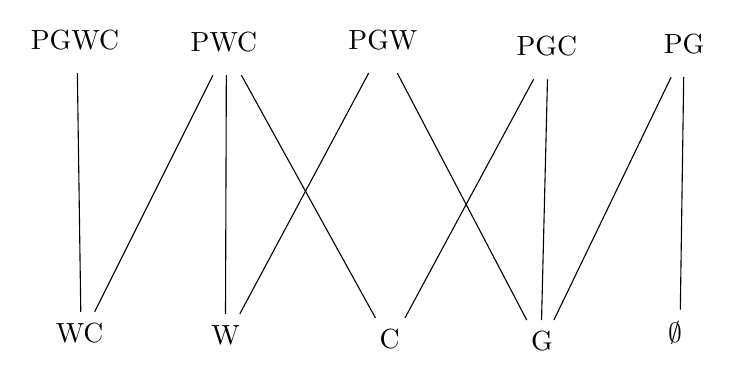
\begin{tikzpicture}[x=0.75pt,y=0.75pt,yscale=-1,xscale=1]
			%uncomment if require: \path (0,236); %set diagram left start at 0, and has height of 236
	
	
			% Text Node
			\draw (3,5.4) node [anchor=north west][inner sep=0.75pt]    {$\text{PGWC}$};
			% Text Node
			\draw (15,146.4) node [anchor=north west][inner sep=0.75pt]    {$\text{WC}$};
			% Text Node
			\draw (80,6.4) node [anchor=north west][inner sep=0.75pt]    {$\text{PWC}$};
			% Text Node
			\draw (90,147.4) node [anchor=north west][inner sep=0.75pt]    {$\text{W}$};
			% Text Node
			\draw (156,5.4) node [anchor=north west][inner sep=0.75pt]    {$\text{PGW}$};
			% Text Node
			\draw (171,149.4) node [anchor=north west][inner sep=0.75pt]    {$\text{C}$};
			% Text Node
			\draw (244,150.4) node [anchor=north west][inner sep=0.75pt]    {$\text{G}$};
			% Text Node
			\draw (237,8.4) node [anchor=north west][inner sep=0.75pt]    {$\text{PGC}$};
			% Text Node
			\draw (308,7.4) node [anchor=north west][inner sep=0.75pt]    {$\text{PG}$};
			% Text Node
			\draw (310,145.4) node [anchor=north west][inner sep=0.75pt]    {$\emptyset $};
			% Connection
			\draw    (26.68,27) -- (28.32,142) ;
			% Connection
			\draw    (35,142) -- (92,28) ;
			% Connection
			\draw    (98.45,28) -- (98.05,143) ;
			% Connection
			\draw    (104.96,143) -- (167.04,27) ;
			% Connection
			\draw    (180.81,27) -- (243.19,146) ;
			% Connection
			\draw    (256.27,146) -- (312.73,29) ;
			% Connection
			\draw    (318.81,29) -- (317.18,141) ;
			% Connection
			\draw    (105.68,28) -- (170.32,145) ;
			% Connection
			\draw    (184.51,145) -- (246.49,30) ;
			% Connection
			\draw    (253.18,30) -- (250.32,146) ;
			\end{tikzpicture}
		\end{center}

		And it's easy to solve now! 

	\end{frame}

	\begin{frame}
		\frametitle{Why Abstraction?}
		\framesubtitle{Easy to Maintain}
		(II) Easy to Maintain
		
		Black-box abstraction: What is it about.

		\begin{example}
			We have AND gates and NOT gates and so on...
			\pause

			We have some wires to construct a functional logic gate.
			\begin{center}
				
				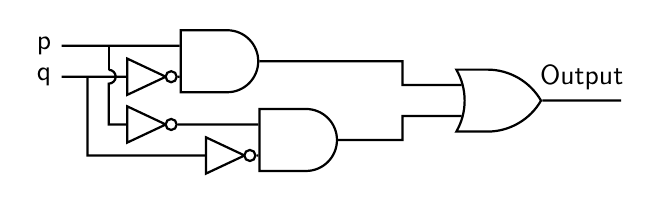
\begin{tikzpicture}[
					%Environment config
					font=\sffamily,
					thick,
					scale=0.5,
					%Environment styles
					GateCfg/.style={
						logic gate inputs={normal,normal,normal},
						draw,
						scale=1
					}
					][
					\path
					(0,0) node[and gate US,GateCfg](AND1){} 
					++ (2,-2) node[and gate US,GateCfg](AND2){} 
					++ (5,1) node[or gate US,GateCfg](OR1){}
					(AND1.input 3)
					++ (-1,0) node[not gate US, draw](N1){}
					(AND2.input 3)
					++ (-1,0) node[not gate US, draw](N2){}
					(AND2.input 1 -| N1)
					node[not gate US, draw](N3){};
					
					\draw
					(OR1.input 1) -- ++(-1.5,0) |- (AND1.output)
					(OR1.input 3) -- ++(-1.5,0) |- (AND2.output)
					(N2.output)--(AND2.input 3)
					(N1.output)--(AND1.input 3)
					(N3.output)--(AND2.input 1)
					(AND1.input 1) 
					-- ++(-3,0) coordinate (init) node[anchor=east]{p}
					node[pos=0.6](temp){}
					(N1-| temp)
					++(0,5pt) edge (temp.center)
					arc (90:-90:5pt) |- (N3.input)
					(init |- N1) node[anchor=east]{q} 
					-- (N1.input) node[pos=0.4](temp2){}
					(temp2.center) |- (N2.input)
					(OR1.output) -- ++(2,0) node [midway,anchor=south]{Output};
				\end{tikzpicture} 
			\end{center} 
		\end{example}

		
		
	
	\end{frame}
	\begin{frame}
		\frametitle{Why Abstraction?}
		\framesubtitle{Easy to Maintain}
		Black-box abstraction: More precisely...
		\begin{itemize}
			\item Basic Elements: something that are pretty basic.(like sets in Maths)
			\item Means of Combination: may construct something rather complicated(composition of functions, etc.)
			\item Means of Abstraction: investigate how can we abstract things(like fixed patterns in math problems)
			\item Capturing Common Patterns: find how we make the abstractions (like reflection and summarizing after solving a problems)
		\end{itemize}

		The black-box abstraction uses the idea of abstraction itself!
	
		
	\end{frame}

	\begin{frame}
		\frametitle{Why Abstraction?}
		\framesubtitle{Friendly to represent Data}
		
		(III) Friendly to represent Data

		machine to automate things $\rightarrow$ computers 

		\begin{itemize}
			\item state of \textbf{automation machine} is limited
			\item a ``translation'' from real-world problems to \textbf{automation machine}
		\end{itemize}

		\begin{figure}
			\includegraphics[scale=0.2]{turing-machine.png}
		\end{figure}
	
	\end{frame}

	\begin{frame}
		\frametitle{How to Abstract?}
	
		\begin{center}
			\Huge{Algorithms' Help}
		\end{center}
	
	\end{frame}

	\subsection{Algorithms}

	\begin{frame}
		\frametitle{Make ``abstractions'' dynamic}
		
		Find the page of word $s$ in \textit{Oxford Advanced Learners' Dictionary}
		
		\pause

		\begin{example}[Find the page of word $s$(assuming no spelling mistakes) in OALD]
			\small
			\textbf{Algorithm 1.}
			
			for \textit{word} in \textit{dictionary}, 

			\qquad if \textit{word} is equal to \textit{s},

			\qquad \qquad return the page of \textit{s}
			
			\pause

			\textbf{Algorithm 2.}
			
			\textit{find word} in (\textit{start page}, \textit{end page})
			
			Open to the \textit{middle}($\lfloor (startpage+endpage)/2 \rfloor$)
			
			\qquad Look at page
			
			\qquad If the word is on the page, return the page number.
			
			\qquad If the word is earlier in the dictionary, \textit{find word} in(\textit{start page}, \textit{middle})
		
			\qquad If the word is later in the dictionary, \textit{find word} in (\textit{middle}+1, \textit{end page})
			
		\end{example}		
	
	\end{frame}

	\begin{frame}
		\frametitle{That's it}
	
		But make sure that you have proved$\dots$

		\begin{itemize}
			\item your algorithm is correct
			\item your algorithm is (somehow) optimized
		\end{itemize}
	
	\end{frame}

	\section{Application}
	
	\begin{frame}
		\frametitle{ETC System}
		
		Efforts made in the field of abstraction and algorithms
		\begin{itemize}
			\item huge \textbf{database} system $\rightarrow$ Abstraction(II) (III)
			\begin{itemize}
				\item data racing, concurrency problems $\rightarrow$ (Algorithm )
				\item efficiency $\rightarrow$(Algorithm )
			\end{itemize}
			\item signals received by receiver $\rightarrow$ Abstraction(I), (III)

		\end{itemize}
	
	\end{frame}

	\begin{frame}
		\frametitle{Automation Production in Factory}
		
		Efforts made in the field of abstraction and algorithms
		\begin{itemize}
			\item simulation process $\rightarrow$ Abstraction(I, II)
			\item stabilize the body of the robots $\rightarrow$ Algorithm 

		\end{itemize}
	
	\end{frame}

	\begin{frame}
		\frametitle{Dish washing}
		
		Efforts made in the field of abstraction and algorithms
		\begin{itemize}
			\item the ``washing process'' $\rightarrow$ Algorithm 
			\item the construct of the machine $\rightarrow$ Abstraction(II)

		\end{itemize}
	
	\end{frame}

	\begin{frame}
		\frametitle{Verify Mathematical Proofs}
		
		Efforts made in the field of abstraction and algorithms
		\begin{itemize}
			\item rules about logic $\rightarrow$ Abstraction(I)
			\begin{itemize}
				\item if $p$ is a prop. , $\neg \neg p \leftrightarrow p$
				\item $A\wedge (B\wedge C) = (A\wedge B)\wedge C$
				\item ...
			\end{itemize}

		\end{itemize}

		\textit{Lean Theorem Prover}

		\url{http://leanprover-community.github.io/lean-web-editor}

		
	
	\end{frame}

	\begin{frame}[fragile=singleslide]
		\frametitle{Verify Mathematical Proofs}
		\begin{example}
			\begin{verbatim}
				variables A B C D : Prop
				variable h1 : A -> B -> C
				variable h2 : D -> A
				variable h3 : D
				variable h4 : B
				#check h2 h3
				#check h1 (h2 h3)
				#check h1 (h2 h3) h4
			\end{verbatim}
		\end{example}
	
	More stuff: \url{https://leanprover.github.io/theorem_proving_in_lean4/title_page.html}
	
	\end{frame}

	\begin{frame}
		\frametitle{Data Providers on Web}

		gets information by...
		\begin{itemize}
			\item web crawler
			\item government files
			\item official dataset
		\end{itemize}

		before automatically process these data.
	
		
	
	\end{frame}

	\section*{Thanks and acknowledgements}


	\begin{frame}
		\frametitle{Summary and References}
	
		[1] \textit{Problem Solving 2020}, Nanjing University.
		
		[2] \textit{Minecraft Logic Gates}, FandomWiki.

		[3] \textit{Structure and Interpretation of Computer Programs, 1986}, MIT.
		
		[4] \textit{CS50x 2022}, Harvard University.
		
		[5] \textit{Logic and Proof} by Jeremy Avigad, Robert Y. Lewis, and Floris van Doorn.
	
	\end{frame}

	\begin{frame}
		
		$$\Huge \text{Thanks!}$$
	\end{frame}
	
\end{document}